\chapter{Estereoquímica en profundidad}\label{ch:b1:stereochemistry-in-depth}

Tritúrense unas semillas de alcaravea y, después, una hoja de
hierbabuena: dos olores muy distintos. El odorante principal de cada una
es la carvona, \ce{C10H14O}, los mismos átomos unidos en el mismo orden
--- pero las dos carvonas son imágenes especulares la una de la otra,
como una mano izquierda lo es de una derecha, y los receptores de la
nariz, construidos a su vez con moléculas asimétricas respecto del
espejo, las distinguen. Los medicamentos, los aromas y las moléculas de
la vida están construidos en tres dimensiones, y una fórmula estructural
que ignora la tercera dimensión se deja la mitad de la historia. Este
capítulo da las herramientas para dibujar las moléculas en el espacio,
nombrar cada disposición sin ambigüedad, seguir las rotaciones que las
moléculas realizan constantemente y medir la única propiedad física que
distingue las imágenes especulares.

\begin{recall}
El volumen escolar (año 12) introdujo las moléculas \omterm{def:b1:stereochemistry-in-depth:stereocentre}{quirales}, el carbono
asimétrico, los \omterm{def:b1:stereochemistry-in-depth:enantiomers}{enantiómeros}, los isómeros $Z$/$E$ y las \omterm{def:b1:stereochemistry-in-depth:isomers}{conformaciones}
del etano. La disposición tetraédrica de los cuatro enlaces alrededor del
carbono y la descripción $\sigma$/$\pi$ de los enlaces sencillos y dobles
proceden del
\cref{ch:b1:lewis-resonance-vsepr}.
\end{recall}

\begin{omfigure}
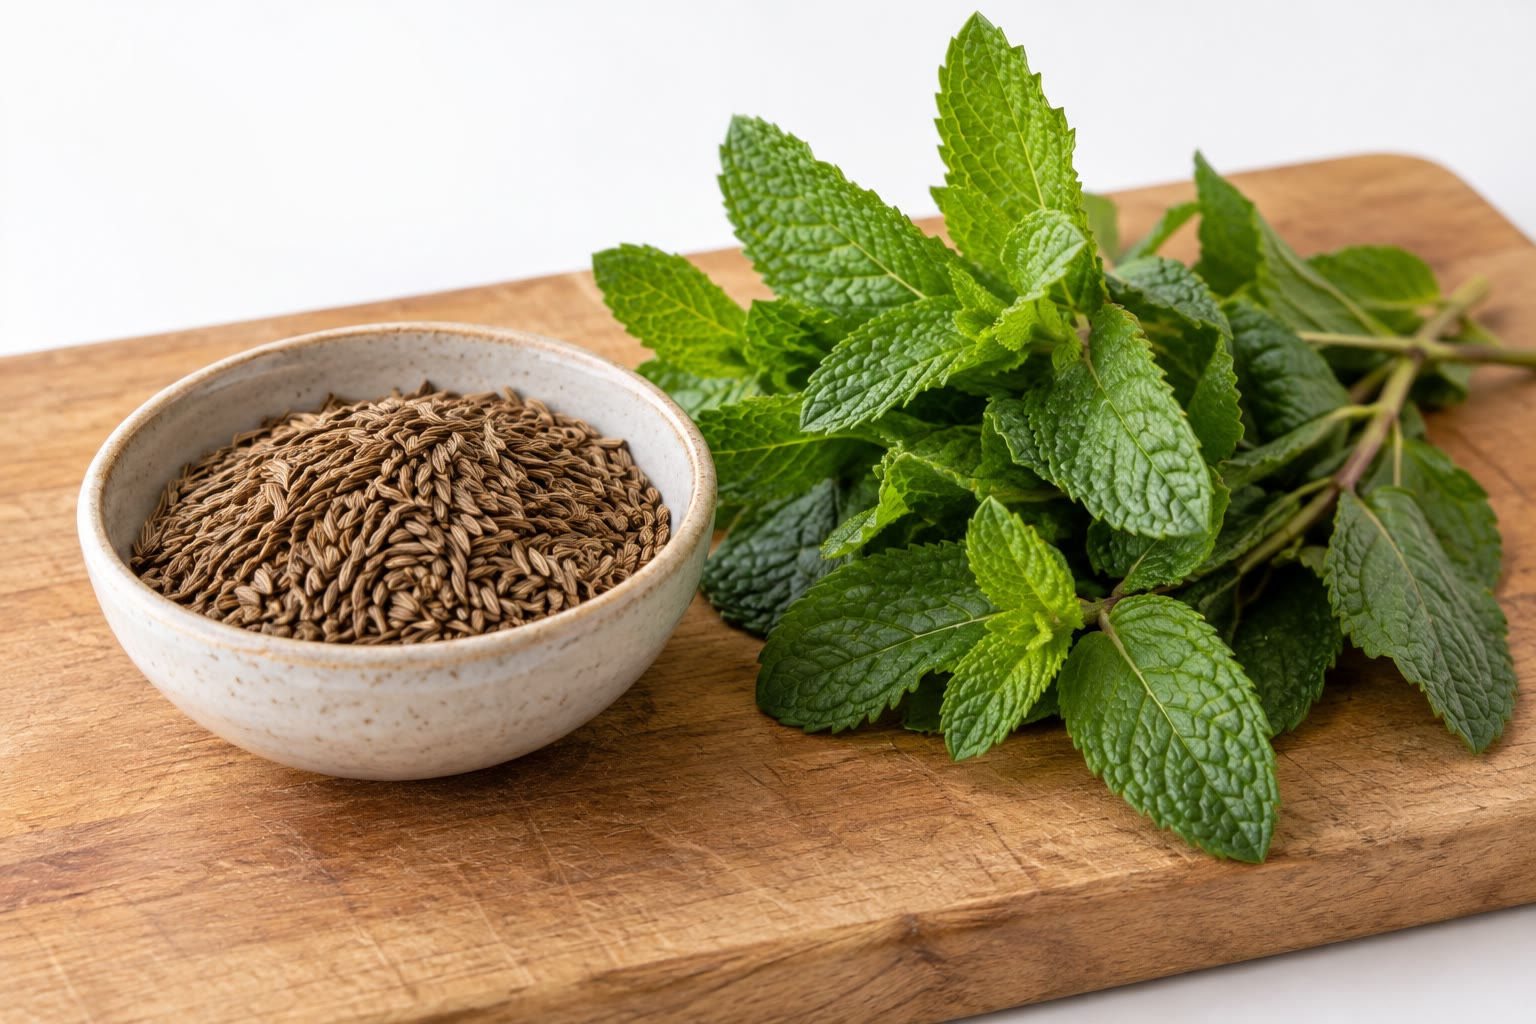
\includegraphics[width=0.55\linewidth]{images/book2/ai/b1-16-caraway-mint.jpg}

{\small Semillas de alcaravea y hojas de hierbabuena. La alcaravea debe su
olor sobre todo a la \cip{S}-carvona, y la hierbabuena, a su imagen
especular, la \cip{R}-carvona.}
\end{omfigure}

\section{Isómeros y representaciones}

\begin{definition}[Constitución, configuración, conformación]\label{def:b1:stereochemistry-in-depth:isomers}
Dos compuestos de la misma fórmula cuyos átomos están unidos en un orden
distinto son \emph{isómeros constitucionales}\index{isomeros constitucionales@isómeros constitucionales}.
Los compuestos de la misma constitución cuyos átomos solo difieren en su
disposición en el espacio son \emph{estereoisómeros}\index{estereoisomeros@estereoisómeros}. La
disposición que solo puede cambiarse rompiendo enlaces es la
\emph{configuración}\index{configuracion@configuración} de un estereoisómero; una disposición
obtenida por rotación alrededor de enlaces sencillos, sin romper ninguno,
es una \emph{conformación}\index{conformacion@conformación}.
\end{definition}

A temperatura ambiente, las rotaciones alrededor de los enlaces sencillos
se producen miles de millones de veces por segundo: las \omterm{def:b1:stereochemistry-in-depth:isomers}{conformaciones} se
interconvierten y no pueden aislarse, mientras que las \omterm{def:b1:stereochemistry-in-depth:isomers}{configuraciones}
son estables y dan compuestos distintos.

\begin{definition}[Representaciones]\label{def:b1:stereochemistry-in-depth:representations}
En la \emph{representación de Cram}\index{representacion de Cram@representación de Cram} se dibujan dos
enlaces en el plano de la página, una cuña llena apunta hacia el lector y
una cuña rayada, en sentido contrario. Una \emph{proyección de
Newman}\index{proyeccion de Newman@proyección de Newman} mira una molécula a lo largo de un enlace
C--C: el carbono delantero es un punto en el que se unen sus otros tres
enlaces, y el carbono trasero, un círculo de cuyo borde salen sus
enlaces. En una \emph{proyección de Fischer}\index{proyeccion de Fischer@proyección de Fischer}
la cadena carbonada es vertical, los enlaces horizontales apuntan hacia el
lector y los verticales en sentido contrario; cada cruce es un carbono
estereogénico.
\end{definition}

\begin{omfigure}
\begin{tikzpicture}[font=\small]
  % staggered and eclipsed ethane, Newman
  \pic (s) at (0,0) {omnewman={90}{30}};
  \foreach \k in {1,2,3} { \node at (s-f\k) {H}; \node at (s-b\k) {H}; }
  \node at (0,-1.9) {alternada};
  \pic (e) at (3.6,0) {omnewman={90}{108}};
  \foreach \k in {1,2,3} { \node at (e-f\k) {H}; }
  \foreach \k in {1,2,3} { \node[font=\scriptsize, black!60] at ($(e-b\k)!-0.12!(e-c)$) {H}; }
  \node at (3.6,-1.9) {eclipsada};
  % Fischer projection of (R)-lactic acid
  \begin{scope}[xshift=7.6cm]
    \draw[thick] (-0.9,0) -- (0.9,0) (0,-0.9) -- (0,0.9);
    \node[above] at (0,0.9) {\ce{COOH}};
    \node[below] at (0,-0.9) {\ce{CH3}};
    \node[left] at (-0.9,0) {H};
    \node[right] at (0.9,0) {OH};
    \node at (0,-1.9) {Fischer};
  \end{scope}
  % Cram of the same
  \begin{scope}[xshift=11.0cm]
    \node at (0,0) {\chemfig{C(-[2]COOH)(-[:210]H_3C)(<:[:-12]OH)(<[:-55]H)}};
    \node at (0,-1.9) {Cram};
  \end{scope}
\end{tikzpicture}

{\small A la izquierda, \omterm{def:b1:stereochemistry-in-depth:representations}{proyecciones de Newman} del etano a lo largo de su
enlace C--C, alternada (enlaces traseros entre los delanteros) y
eclipsada (enlaces traseros ocultos detrás de los delanteros, dibujados
ligeramente desplazados). A la derecha, la misma molécula, el ácido
\cip{R}-láctico, en \omterm{def:b1:stereochemistry-in-depth:representations}{proyección de Fischer} y en \omterm{def:b1:stereochemistry-in-depth:representations}{representación de Cram}
(los enlaces verticales de la cruz de Fischer se alejan del lector, y los
horizontales se acercan a él).}
\end{omfigure}

\begin{method}[De Cram a Newman]\label{met:b1:stereochemistry-in-depth:newman-from-cram}
\begin{enumerate}
  \item Se elige el enlace a lo largo del cual se mira y el extremo más
        cercano al ojo.
  \item Se dibujan desde el centro los tres enlaces del carbono
        delantero, conservando su orden (en el sentido de las agujas del
        reloj o en el contrario) tal como se ve desde el ojo.
  \item Se dibujan desde el círculo los enlaces del carbono trasero, con
        su orden visto desde el mismo lado.
  \item Comprobación: girar el carbono trasero $60^\circ$ hace pasar de
        alternada a eclipsada; girarlo $120^\circ$, de una \omterm{def:b1:stereochemistry-in-depth:conformations}{conformación
        alternada} a la siguiente.
\end{enumerate}
\end{method}

\section{Configuración: las reglas CIP}

\begin{definition}[Reglas CIP, descriptores]\label{def:b1:stereochemistry-in-depth:cip}
Las \emph{reglas CIP}\index{reglas CIP} (Cahn--Ingold--Prelog) ordenan los
cuatro sustituyentes de un \omterm{def:b1:stereochemistry-in-depth:stereocentre}{centro estereogénico}: primero el de mayor
número atómico; en caso de empate, se comparan los conjuntos de átomos
unidos a continuación, y así sucesivamente hacia fuera; un enlace doble
cuenta como dos enlaces sencillos a átomos duplicados. Con el
sustituyente de menor prioridad alejado del ojo, la secuencia
$1 \to 2 \to 3$ girando en el sentido de las agujas del reloj define el
descriptor \cip{R}, y en sentido contrario, \cip{S}. Para un enlace doble
con dos sustituyentes en cada carbono, \cip{Z} significa que los dos de
mayor prioridad están del mismo lado, y \cip{E}, en lados opuestos.
\end{definition}

\begin{method}[Asignar \texorpdfstring{\cip{R}}{(R)} o \texorpdfstring{\cip{S}}{(S)}]\label{met:b1:stereochemistry-in-depth:cip}
\begin{enumerate}
  \item Se ordenan los cuatro sustituyentes según las \omterm{def:b1:stereochemistry-in-depth:cip}{reglas CIP}.
  \item Si el de menor prioridad se aleja del observador (cuña rayada, o
        enlace vertical de una \omterm{def:b1:stereochemistry-in-depth:representations}{proyección de Fischer}), se lee
        directamente el giro de $1 \to 2 \to 3$.
  \item Si se acerca al observador (cuña llena, enlace horizontal de
        Fischer), se lee el giro y se invierte el descriptor.
  \item Intercambiar dos sustituyentes cualesquiera invierte el
        descriptor: una comprobación rápida.
\end{enumerate}
En el ácido láctico, $\ce{OH} > \ce{COOH} > \ce{CH3} > \ce{H}$ (O; después,
C(O,O,O) gana a C(H,H,H)). En la \omterm{def:b1:stereochemistry-in-depth:representations}{proyección de Fischer} de arriba, H es
horizontal (hacia nosotros) y $\ce{OH} \to \ce{COOH} \to \ce{CH3}$ gira en
sentido contrario a las agujas del reloj: invertido, el centro es
\cip{R}.
\end{method}

\section{La quiralidad y sus consecuencias}

\begin{definition}[Centro estereogénico, quiralidad]\label{def:b1:stereochemistry-in-depth:stereocentre}
Un objeto es \emph{quiral}\index{quiral} si no puede superponerse a su
imagen especular, y \emph{aquiral}\index{aquiral} en caso contrario; la
propiedad es la \emph{quiralidad}\index{quiralidad}. Un \emph{centro
estereogénico}\index{centro estereogenico@centro estereogénico} es un átomo en el que intercambiar
dos sustituyentes da un estereoisómero; un carbono tetraédrico con cuatro
sustituyentes distintos lo es.
\end{definition}

Una molécula con un plano de simetría o un centro de simetría es \omterm{def:b1:stereochemistry-in-depth:stereocentre}{aquiral};
una molécula sin ninguno de los dos es \omterm{def:b1:stereochemistry-in-depth:stereocentre}{quiral} en la práctica. El criterio
exacto, en términos de operaciones de simetría, se da en el volumen del
tercer año.

\begin{definition}[Enantiómeros, diastereoisómeros, compuesto meso, mezcla racémica]\label{def:b1:stereochemistry-in-depth:enantiomers}
Dos \omterm{def:b1:stereochemistry-in-depth:isomers}{estereoisómeros} que son imágenes especulares el uno del otro son
\emph{enantiómeros}\index{enantiomeros@enantiómeros}; los \omterm{def:b1:stereochemistry-in-depth:isomers}{estereoisómeros} que no lo son son
\emph{diastereoisómeros}\index{diastereoisomeros@diastereoisómeros}. Un \emph{compuesto
meso}\index{compuesto meso} tiene \omterm{def:b1:stereochemistry-in-depth:stereocentre}{centros estereogénicos} pero es \omterm{def:b1:stereochemistry-in-depth:stereocentre}{aquiral}.
Una mezcla equimolar de dos enantiómeros es una \emph{mezcla
racémica}\index{mezcla racemica@mezcla racémica}.
\end{definition}

\begin{proposition}[Número de estereoisómeros]\label{prop:b1:stereochemistry-in-depth:max-stereoisomers}
Una molécula con $n$ \omterm{def:b1:stereochemistry-in-depth:stereocentre}{centros estereogénicos} (y ninguna otra unidad
estereogénica) tiene como máximo $2^n$ \omterm{def:b1:stereochemistry-in-depth:isomers}{estereoisómeros}, en como máximo
$2^{n-1}$ parejas de \omterm{def:b1:stereochemistry-in-depth:enantiomers}{enantiómeros}; las formas meso reducen ese número.
\end{proposition}

\begin{proof}
Cada centro es \cip{R} o \cip{S} de forma independiente: $2^n$
combinaciones. La imagen especular cambia todos los descriptores, de modo
que las combinaciones se agrupan en parejas de \omterm{def:b1:stereochemistry-in-depth:enantiomers}{enantiómeros}, $2^{n-1}$
parejas. Si una combinación es su propia imagen especular tras una
rotación de la molécula (una forma meso), su pareja se reduce a un solo
compuesto.
\end{proof}

El ácido tartárico, \ce{HOOC-CH(OH)-CH(OH)-COOH}, tiene dos centros
equivalentes: \cip{R,R} y \cip{S,S} son \omterm{def:b1:stereochemistry-in-depth:enantiomers}{enantiómeros}, mientras que
\cip{R,S} tiene un plano especular entre los dos carbonos y es meso: tres
\omterm{def:b1:stereochemistry-in-depth:isomers}{estereoisómeros}, no cuatro.

\begin{proposition}[Propiedades de los enantiómeros]\label{prop:b1:stereochemistry-in-depth:enantiomer-properties}
Dos \omterm{def:b1:stereochemistry-in-depth:enantiomers}{enantiómeros} tienen los mismos puntos de fusión y de ebullición, las
mismas \omterm{def:b1:precipitation:solubility}{solubilidades} en disolventes \omterm{def:b1:stereochemistry-in-depth:stereocentre}{aquirales}, los mismos espectros y la
misma reactividad frente a reactivos \omterm{def:b1:stereochemistry-in-depth:stereocentre}{aquirales}; difieren en su acción
sobre la luz polarizada y en sus interacciones con otras moléculas
\omterm{def:b1:stereochemistry-in-depth:stereocentre}{quirales}. Los \omterm{def:b1:stereochemistry-in-depth:enantiomers}{diastereoisómeros} difieren en todas sus propiedades.
\end{proposition}

\begin{proof}
Toda propiedad que solo depende de distancias y ángulos dentro de la
molécula, o entre ella y participantes \omterm{def:b1:stereochemistry-in-depth:stereocentre}{aquirales}, es la misma para un
objeto y su imagen especular, ya que una reflexión conserva distancias y
ángulos. Un participante \omterm{def:b1:stereochemistry-in-depth:stereocentre}{quiral} (un receptor, un reactivo \omterm{def:b1:stereochemistry-in-depth:stereocentre}{quiral}, la
trayectoria helicoidal de la luz polarizada descrita más abajo) forma
parejas diastereoisómeras, que ya no son imágenes especulares y, por
tanto, difieren. Los \omterm{def:b1:stereochemistry-in-depth:enantiomers}{diastereoisómeros} no están relacionados por ninguna
reflexión: sus distancias internas difieren.
\end{proof}

\begin{omfigure}
\begin{tikzpicture}[font=\small, line join=round]
  \foreach \dx/\kind/\lab in {0/1/{\cip{R}-carvona (hierbabuena)}, 5.2/0/{\cip{S}-carvona (alcaravea)}} {
  \begin{scope}[xshift=\dx cm]
    \coordinate (c1) at (0,1); \coordinate (c2) at (0.87,0.5);
    \coordinate (c3) at (0.87,-0.5); \coordinate (c4) at (0,-1);
    \coordinate (c5) at (-0.87,-0.5); \coordinate (c6) at (-0.87,0.5);
    \draw[thick] (c1) -- (c2) -- (c3) -- (c4) -- (c5) -- (c6) -- cycle;
    \draw[thick] ($(c2)!0.15!(c3)+(-0.12,0)$) -- ($(c3)!0.15!(c2)+(-0.12,0)$);
    \draw[thick] (c1) -- ++(0,0.7) node[above] {O};
    \draw[thick] ($(c1)+(0.1,0)$) -- ++(0,0.62);
    \draw[thick] (c2) -- ++(0.75,0.43) node[right] {\ce{CH3}};
    \coordinate (q) at ($(c5)+(-0.75,-0.43)$);
    \ifnum\kind=1
      \fill (c5) -- ($(q)+(0.06,-0.1)$) -- ($(q)+(-0.06,0.1)$) -- cycle;
    \else
      \foreach \t in {0.15,0.3,0.45,0.6,0.75,0.9}
        \draw ($(c5)!\t!(q)+(\t*0.06,-\t*0.1)$) -- ($(c5)!\t!(q)+(-\t*0.06,\t*0.1)$);
    \fi
    \draw[thick] (q) -- ++(-0.6,0.5) node[above] {\ce{CH2}};
    \draw[thick] ($(q)+(0.08,0.06)$) -- ++(-0.6,0.5);
    \draw[thick] (q) -- ++(0,-0.75) node[below] {\ce{CH3}};
    \node[font=\scriptsize] at ($(c5)+(0.35,0.12)$) {5};
    \node at (0,-2.85) {\lab};
  \end{scope}}
\end{tikzpicture}

{\small Las dos carvonas, dibujadas sobre el mismo esqueleto: el grupo
isopropenilo de C5 apunta hacia el lector (cuña llena) en una y se aleja
de él (cuña rayada) en la otra, con el hidrógeno de C5 (no dibujado) del
lado opuesto. Son imágenes especulares la una de la otra: \omterm{def:b1:stereochemistry-in-depth:enantiomers}{enantiómeros}
(\cref{exo:b1:stereochemistry-in-depth:4}).}
\end{omfigure}

\begin{history}[Un carbono tetraédrico]
\begin{minipage}[t]{0.2\linewidth}\vspace{0pt}
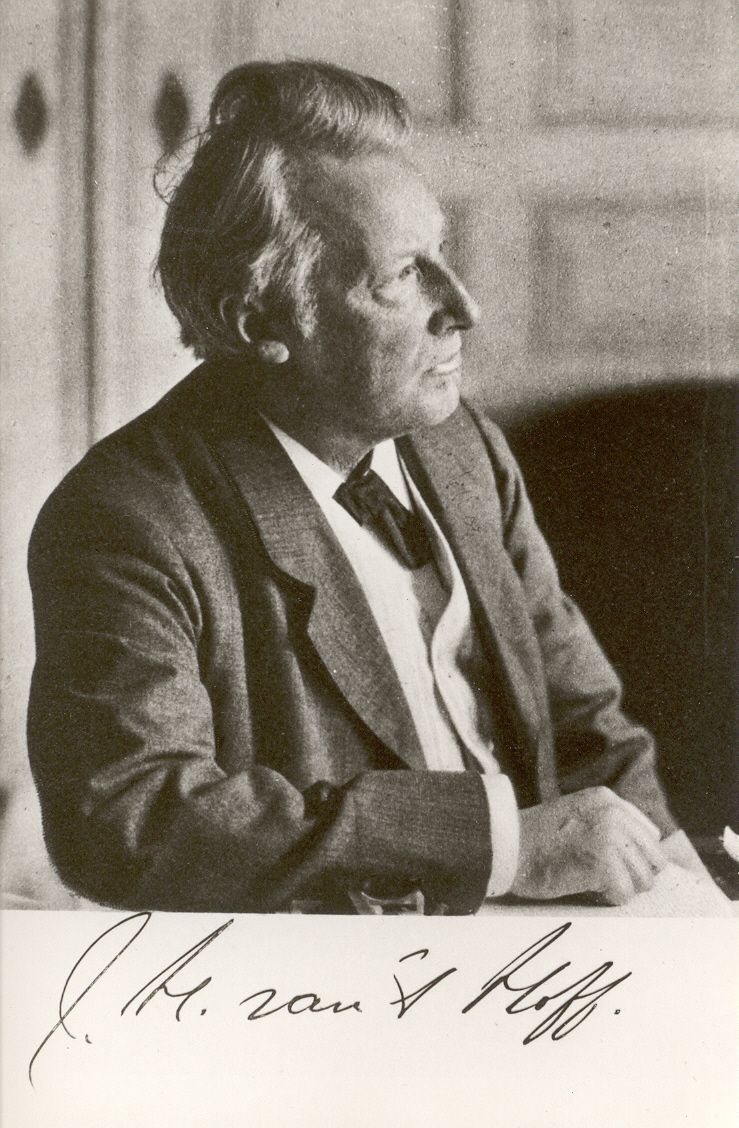
\includegraphics[width=\linewidth]{images/book2/van-t-hoff.jpg}
\end{minipage}\hfill
\begin{minipage}[t]{0.76\linewidth}\vspace{0pt}
Jacobus Henricus van 't Hoff propuso, siendo un químico joven, que los
cuatro enlaces de un átomo de carbono apuntan a los vértices de un
tetraedro. Un carbono con cuatro sustituyentes distintos existe entonces
como dos disposiciones especulares, lo que explicaba por qué algunos
compuestos se presentan en dos formas que solo difieren en el sentido en
que giran la luz polarizada. La idea es el punto de partida de todos los
dibujos de este capítulo.
(Fotografía publicada en 1911, dominio público, Wikimedia Commons.)
\end{minipage}
\end{history}

\section{Conformaciones}

\begin{definition}[Ángulo de torsión y conformaciones]\label{def:b1:stereochemistry-in-depth:conformations}
Para cuatro átomos A--B--C--D, el \emph{ángulo de torsión}\index{angulo de torsion@ángulo de torsión}
$\theta$ alrededor de B--C es el ángulo entre los planos ABC y BCD, que
se lee en una \omterm{def:b1:stereochemistry-in-depth:representations}{proyección de Newman} a lo largo de B--C. Una \omterm{def:b1:stereochemistry-in-depth:isomers}{conformación} es
una \emph{conformación eclipsada}\index{conformacion eclipsada@conformación eclipsada} cuando los enlaces de
los carbonos delantero y trasero están alineados en la proyección, y una
\emph{conformación alternada}\index{conformacion alternada@conformación alternada} cuando se alternan.
En el butano, visto a lo largo de C2--C3, la \omterm{def:b1:stereochemistry-in-depth:isomers}{conformación} alternada con
los dos grupos metilo a $180^\circ$ es la \emph{conformación anti}\index{conformacion anti@conformación anti},
y las que los tienen a $\pm 60^\circ$ son \emph{conformaciones
gauche}\index{conformacion gauche@conformación gauche}. En el ciclohexano, el anillo plegado sin
tensión es la \emph{silla}\index{silla}; cada carbono lleva un enlace
\emph{axial}\index{axial}, paralelo al eje del anillo, y un enlace
\emph{ecuatorial}\index{ecuatorial}, aproximadamente en el plano medio del
anillo. La \emph{inversión del anillo}\index{inversion del anillo@inversión del anillo} convierte
una silla en la otra: todo enlace axial pasa a ser ecuatorial, y a la
inversa.
\end{definition}

\begin{omfigure}
\begin{tikzpicture}
\begin{axis}[
  width=0.82\linewidth, height=5.8cm, xmin=0, xmax=360, ymin=0, ymax=21,
  legend style={font=\scriptsize, draw=none, at={(0.5,0.62)}, anchor=center},
  axis x line=bottom, axis y line=left, xlabel={ángulo de torsión $\theta$ (grados)},
  ylabel={energía (kJ/mol)}, xtick={0,60,120,180,240,300,360},
  tick label style={font=\small}, label style={font=\small}]
\addplot[omDef, very thick] table[x=theta, y=butane] {figdata/out/bachelor-1-butane-torsion.dat};
\addplot[omProp, thick, dashed] table[x=theta, y=ethane] {figdata/out/bachelor-1-butane-torsion.dat};
\node[font=\scriptsize, anchor=south west] at (axis cs:0,18.4) {sin};
\node[font=\scriptsize, anchor=south] at (axis cs:62,18.4) {gauche};
\node[font=\scriptsize, anchor=south] at (axis cs:120,18.4) {eclipsada};
\node[font=\scriptsize, anchor=south] at (axis cs:180,18.4) {anti};
\node[font=\scriptsize, anchor=south] at (axis cs:240,18.4) {eclipsada};
\node[font=\scriptsize, anchor=south] at (axis cs:298,18.4) {gauche};
\node[font=\scriptsize, anchor=south east] at (axis cs:360,18.4) {sin};
\legend{butano, etano}
\end{axis}
\end{tikzpicture}

{\small Energía de torsión del butano alrededor de su enlace central
(continua; $\theta
= 0$ cuando los grupos metilo se eclipsan) y del etano
(discontinua), calculadas a partir de potenciales de torsión
experimentales. Etano: barrera de \qty{12.2}{kJ/mol}. Butano: la anti es
la más estable; la gauche está \qty{2.8}{kJ/mol} más arriba, en
$\theta = 62^\circ$; barreras de \qty{15.2}{kJ/mol} (metilo eclipsando
hidrógeno) y de \qty{16.5}{kJ/mol} (metilo eclipsando metilo).}
% ledger: rot:ethane-V3, rot:butane-V1, rot:butane-V2, rot:butane-V3, rot:butane-V4, rot:butane-V5, rot:butane-V6 (curves in figdata/bachelor-1/butane-torsion.py)
\end{omfigure}

Las barreras son pequeñas frente a la energía térmica disponible en los
choques ($RT = \qty{2.5}{kJ/mol}$ a temperatura ambiente, y mucho más en
la cola de la distribución, \cref{ch:b1:elementary-steps}): la rotación
es rápida, y el butano es una mezcla de moléculas anti y gauche que no
pueden separarse.

\begin{method}[Dibujar una silla]\label{met:b1:stereochemistry-in-depth:draw-chair}
\begin{enumerate}
  \item Se dibujan dos rectas paralelas ligeramente inclinadas hacia
        abajo a la derecha, desplazadas; se unen sus extremos con una V a
        la izquierda y una V invertida a la derecha para cerrar el anillo
        de seis miembros.
  \item Los enlaces \omterm{def:b1:stereochemistry-in-depth:conformations}{axiales} son verticales: hacia arriba en los carbonos
        que apuntan hacia arriba, hacia abajo en los que apuntan hacia
        abajo, alternando alrededor del anillo.
  \item Los enlaces \omterm{def:b1:stereochemistry-in-depth:conformations}{ecuatoriales} son paralelos a los enlaces del anillo
        situados a un enlace de distancia, y apuntan hacia fuera.
  \item Para invertir el anillo, se dibuja la otra \omterm{def:b1:stereochemistry-in-depth:conformations}{silla}; un sustituyente
        \omterm{def:b1:stereochemistry-in-depth:conformations}{axial} en una es \omterm{def:b1:stereochemistry-in-depth:conformations}{ecuatorial} en la otra.
\end{enumerate}
\end{method}

\begin{omfigure}
\begin{tikzpicture}[font=\small]
  \pic (a) at (0,0) {omchair};
  \foreach \k in {1,2,3,4,5,6} \draw[omProp, thick] (a-c\k) -- (a-a\k);
  \foreach \k in {1,2,3,4,5,6} \draw[omDef, thick] (a-c\k) -- (a-e\k);
  \node[omProp, anchor=south] at (a-a3) {axial};
  \node[omDef, anchor=north] at (a-e5) {ecuatorial};
  \begin{scope}[xshift=4.9cm]
    \pic (b) at (0,0) {omchair};
    \draw[thick] (b-c1) -- (b-e1) node[right] {\ce{CH3}};
    \draw[thick] (b-c1) -- (b-a1) node[above] {H};
    \node at (0,-1.5) {\ce{CH3} ecuatorial};
  \end{scope}
  \draw[<->, thick] (8.1,0) -- (8.8,0) node[midway, above] {inv.};
  \begin{scope}[xshift=10.45cm]
    \pic (c) at (0,0) {omchairflip};
    \draw[thick] (c-c4) -- (c-a4) node[below] {\ce{CH3}};
    \draw[thick] (c-c4) -- (c-e4) node[right] {H};
    \node at (0,-1.5) {\ce{CH3} axial};
  \end{scope}
\end{tikzpicture}

{\small A la izquierda, la \omterm{def:b1:stereochemistry-in-depth:conformations}{silla} del ciclohexano con sus seis enlaces
\omterm{def:b1:stereochemistry-in-depth:conformations}{axiales} (en naranja, alternadamente hacia arriba y hacia abajo) y sus
seis enlaces \omterm{def:b1:stereochemistry-in-depth:conformations}{ecuatoriales} (en azul). A la derecha, las dos \omterm{def:b1:stereochemistry-in-depth:conformations}{sillas} del
metilciclohexano, interconvertidas por la \omterm{def:b1:stereochemistry-in-depth:conformations}{inversión del anillo}; el grupo
metilo es \omterm{def:b1:stereochemistry-in-depth:conformations}{ecuatorial} en una y \omterm{def:b1:stereochemistry-in-depth:conformations}{axial} en la otra.}
\end{omfigure}

\begin{proposition}[Se prefieren los sustituyentes ecuatoriales]\label{prop:b1:stereochemistry-in-depth:chair-substituent}
En un ciclohexano monosustituido, la \omterm{def:b1:stereochemistry-in-depth:conformations}{silla} con el sustituyente \omterm{def:b1:stereochemistry-in-depth:conformations}{ecuatorial}
es la más estable. Para un grupo metilo, la posición \omterm{def:b1:stereochemistry-in-depth:conformations}{axial} añade dos
interacciones gauche con carbonos del anillo, cada una del valor de la del
butano (\qtyrange{2.8}{2.9}{kJ/mol}), unos \qty{5.7}{kJ/mol} en total:
una estimación de la diferencia de energía.
\end{proposition}

\begin{proof}
Visto a lo largo del enlace C1--C2, un metilo \omterm{def:b1:stereochemistry-in-depth:conformations}{axial} en C1 está en gauche
respecto de C3 del anillo; visto a lo largo de C1--C6, respecto de C5:
dos interacciones gauche de tipo butano, que también pueden verse como
la aglomeración del metilo con los hidrógenos \omterm{def:b1:stereochemistry-in-depth:conformations}{axiales} de C3 y C5 (las
interacciones 1,3-diaxiales). Un metilo \omterm{def:b1:stereochemistry-in-depth:conformations}{ecuatorial} está en anti respecto
de C3 y C5. Cada interacción gauche cuesta lo que cuesta en el butano,
\qty{2.8}{kJ/mol} en el potencial de torsión de la figura.
\end{proof}

Con $\Delta E = \qty{5.7}{kJ/mol}$, la razón entre \omterm{def:b1:stereochemistry-in-depth:conformations}{sillas} \omterm{def:b1:stereochemistry-in-depth:conformations}{ecuatoriales} y
\omterm{def:b1:stereochemistry-in-depth:conformations}{axiales} a \qty{25}{\celsius} es $\exp(\Delta E/RT) = 10$: alrededor de un
\qty{91}{\percent} \omterm{def:b1:stereochemistry-in-depth:conformations}{ecuatorial} (\cref{exo:b1:stereochemistry-in-depth:9}).
Los grupos grandes, como el terc-butilo, bloquean el anillo en la \omterm{def:b1:stereochemistry-in-depth:conformations}{silla}
en la que son \omterm{def:b1:stereochemistry-in-depth:conformations}{ecuatoriales}.

\section{Actividad óptica}

\begin{definition}[Actividad óptica, rotación específica]\label{def:b1:stereochemistry-in-depth:optical-activity}
Una sustancia presenta \emph{actividad óptica}\index{actividad optica@actividad óptica} si gira
el plano de polarización de la luz linealmente polarizada que la
atraviesa. Para un observador situado frente a la luz, una sustancia
\emph{dextrógira}\index{dextrogira@dextrógira}, que se escribe $(+)$, lo gira en el sentido
de las agujas del reloj, y una \emph{levógira}\index{levogira@levógira},
$(-)$, en sentido contrario. La \emph{rotación específica}\index{rotacion especifica@rotación específica}
es $[\alpha] = \alpha/(\ell c)$, donde $\alpha$ es el ángulo medido en
grados, $\ell$ la longitud del trayecto en decímetros y $c$ la
concentración en masa en \unit{g/mL}; depende de la longitud de onda
(normalmente la línea amarilla del sodio), de la temperatura y del
disolvente.
\end{definition}

\begin{omfigure}
\begin{tikzpicture}[font=\small, >={Stealth}]
  \fill[yellow!70!orange] (0,0) circle (0.25);
  \node[below] at (0,-0.45) {lámpara};
  \draw[thick] (1.3,-0.7) rectangle (1.45,0.7); \node[below] at (1.37,-0.75) {polarizador};
  \draw[omDef!20, fill=omDef!10] (2.4,-0.45) rectangle (5.6,0.45);
  \node at (4.0,0) {muestra, longitud $\ell$};
  \draw[thick] (6.5,-0.7) rectangle (6.65,0.7); \node[below] at (6.57,-0.75) {analizador};
  \draw (7.6,0) circle (0.3); \node[below] at (7.6,-0.45) {ojo};
  \draw[->, orange!80!black] (0.3,0) -- (1.25,0);
  \draw[->, orange!80!black] (1.5,0) -- (2.35,0);
  \draw[->, orange!80!black] (5.65,0) -- (6.45,0);
  % polarisation planes
  \draw[thick, omThm] (1.9,-0.35) -- (1.9,0.35);
  \draw[thick, omThm] (6.05,-0.33) -- ++(70:0.0) -- (5.93,0.33);
  \draw[->, omThm] (5.75,0.55) arc[start angle=100, end angle=70, radius=0.6];
  \node[omThm, above] at (6.1,0.75) {$\alpha$};
\end{tikzpicture}

{\small Un polarímetro. El polarizador deja pasar la luz que vibra en un
plano; la muestra \omterm{def:b1:stereochemistry-in-depth:stereocentre}{quiral} gira ese plano un ángulo $\alpha$; el analizador
se gira hasta que la luz vuelve a extinguirse, lo que mide $\alpha$.}
\end{omfigure}

\begin{proposition}[Ley de Biot]\label{prop:b1:stereochemistry-in-depth:biot}
Para una disolución diluida de varios solutos ópticamente activos, el
ángulo de rotación es aditivo, $\alpha = \ell\sum_i [\alpha]_i c_i$ (\emph{ley
de Biot}\index{ley de Biot}). Dos \omterm{def:b1:stereochemistry-in-depth:enantiomers}{enantiómeros} tienen \omterm{def:b1:stereochemistry-in-depth:optical-activity}{rotaciones
específicas} opuestas; una \omterm{def:b1:stereochemistry-in-depth:enantiomers}{mezcla racémica} no gira la luz.
\end{proposition}

\begin{proof}
En disolución diluida, cada soluto contribuye de forma independiente, en
proporción al número de moléculas atravesadas, es decir, a $\ell c_i$;
ese es el contenido experimental de la ley. Una reflexión convierte el
sentido de las agujas del reloj en el contrario: la molécula imagen
especular gira el plano el ángulo opuesto, y en una \omterm{def:b1:stereochemistry-in-depth:enantiomers}{mezcla racémica} las
dos contribuciones se anulan.
\end{proof}

Para una mezcla de dos \omterm{def:b1:stereochemistry-in-depth:enantiomers}{enantiómeros} a la concentración total $c$, la
fracción $x$ de la forma $(-)$ da $\alpha = \ell c[\alpha]_{(-)}(x - (1 - x)) =
\ell c[\alpha]_{(-)}(2x - 1)$: medir $\alpha$ da la composición. La
rotación óptica no está ligada de forma sencilla al descriptor: un
compuesto \cip{R} puede ser $(+)$ o $(-)$; la \cip{R}-carvona de la
hierbabuena es \omterm{def:b1:stereochemistry-in-depth:optical-activity}{levógira}.

\section{Ejercicios}

\begin{exercise}[$\star$]\label{exo:b1:stereochemistry-in-depth:1}
Clasifíquese cada pareja como \omterm{def:b1:stereochemistry-in-depth:isomers}{isómeros constitucionales}, \omterm{def:b1:stereochemistry-in-depth:enantiomers}{enantiómeros},
\omterm{def:b1:stereochemistry-in-depth:enantiomers}{diastereoisómeros} o dos \omterm{def:b1:stereochemistry-in-depth:isomers}{conformaciones} de un mismo compuesto: butan-1-ol
y butan-2-ol; \cip{R}- y \cip{S}-butan-2-ol; \cip{Z}- y \cip{E}-but-2-eno;
las \omterm{def:b1:stereochemistry-in-depth:isomers}{conformaciones} anti y gauche del butano; ácido \cip{R,R}- y
\cip{R,S}-tartárico.
\end{exercise}

\begin{exercise}[$\star$]\label{exo:b1:stereochemistry-in-depth:2}
Ordénense según las \omterm{def:b1:stereochemistry-in-depth:cip}{reglas CIP}: \ce{-OH}, \ce{-NH2}, \ce{-CH3}, \ce{-H};
después, \ce{-CH2OH}, \ce{-CHO}, \ce{-COOH}, \ce{-CH(CH3)2}; después,
\ce{-Cl},
\ce{-CH2Cl}, \ce{-CCl3}, \ce{-Br}.
\end{exercise}

\begin{exercise}[$\star$]\label{exo:b1:stereochemistry-in-depth:3}
¿Cuántos \omterm{def:b1:stereochemistry-in-depth:isomers}{estereoisómeros} tienen el 2,3-diclorobutano, el
2-bromo-3-clorobutano y el pentano-2,4-diol? Identifíquense las formas
meso.
\end{exercise}

\begin{exercise}[$\star$]\label{exo:b1:stereochemistry-in-depth:4}
Ordénense según las \omterm{def:b1:stereochemistry-in-depth:cip}{reglas CIP} los cuatro sustituyentes del C5 de la
carvona y compruébense los descriptores dados en la figura de las dos
carvonas (cuña llena: el grupo isopropenilo hacia el lector, H en sentido
contrario).
\end{exercise}

\begin{exercise}[$\star\star$]\label{exo:b1:stereochemistry-in-depth:5}
Dibújense las \omterm{def:b1:stereochemistry-in-depth:representations}{proyecciones de Newman} del butano a lo largo de C2--C3 para
$\theta = 0$, 60, 120 y $180^\circ$ y léanse sus energías en la curva.
¿Qué fracción de las moléculas sería gauche si las energías gauche y anti
fueran iguales?
\end{exercise}

\begin{exercise}[$\star\star$]\label{exo:b1:stereochemistry-in-depth:6}
Dibújese la \omterm{def:b1:stereochemistry-in-depth:representations}{proyección de Fischer} de la \cip{S}-alanina,
\ce{H2N-CH(CH3)-COOH}, con el grupo ácido arriba. ¿De qué lado está el
grupo amino?
\end{exercise}

\begin{exercise}[$\star\star$]\label{exo:b1:stereochemistry-in-depth:7}
Demuéstrese que el \textit{cis}-1,2-dimetilciclohexano tiene un metilo
\omterm{def:b1:stereochemistry-in-depth:conformations}{axial} y otro \omterm{def:b1:stereochemistry-in-depth:conformations}{ecuatorial} en las dos \omterm{def:b1:stereochemistry-in-depth:conformations}{sillas}, mientras que el isómero
\textit{trans} tiene una \omterm{def:b1:stereochemistry-in-depth:conformations}{silla} con ambos \omterm{def:b1:stereochemistry-in-depth:conformations}{ecuatoriales}. ¿Qué isómero es
más estable? Úsese la estimación del capítulo.
\end{exercise}

\begin{exercise}[$\star\star$]\label{exo:b1:stereochemistry-in-depth:8}
Una disolución de un compuesto \omterm{def:b1:stereochemistry-in-depth:stereocentre}{quiral} de \qty{0.100}{g/mL} en un tubo de
\qty{2.00}{dm} gira la luz $+13.2^\circ$. Calcúlese $[\alpha]$. ¿Qué daría
un tubo de \qty{1.00}{dm}? ¿Y el enantiómero a la misma concentración?
\end{exercise}

\begin{exercise}[$\star\star$]\label{exo:b1:stereochemistry-in-depth:9}
Calcúlese, con $\Delta E = \qty{5.7}{kJ/mol}$ y la razón de Boltzmann
$\exp(\Delta E/RT)$, la fracción de \omterm{def:b1:stereochemistry-in-depth:conformations}{sillas} de metilciclohexano con el
metilo \omterm{def:b1:stereochemistry-in-depth:conformations}{ecuatorial} a \qty{25}{\celsius} y a \qty{-50}{\celsius}.
\end{exercise}

\begin{exercise}[$\star\star\star$]\label{exo:b1:stereochemistry-in-depth:10}
Explíquese por qué el etano tiene un solo tipo de \omterm{def:b1:stereochemistry-in-depth:conformations}{conformación alternada}
y el butano dos (anti y gauche), y por qué la gauche es menos estable.
Con las energías de la figura, estímese la razón de poblaciones anti :
gauche del butano a \qty{25}{\celsius} (dos \omterm{def:b1:stereochemistry-in-depth:conformations}{conformaciones gauche}, una
anti).
\end{exercise}

\begin{exercise}[$\star\star\star$]\label{exo:b1:stereochemistry-in-depth:11}
Considérese el ácido 2,3,4-trihidroxipentanodioico,
\ce{HOOC-CH(OH)-CH(OH)-CH(OH)-COOH}. Cuéntense sus \omterm{def:b1:stereochemistry-in-depth:stereocentre}{centros
estereogénicos}, demuéstrese que el carbono central solo es estereogénico
cuando los dos externos tienen descriptores opuestos
(pseudoasimétrico), y cuéntense los \omterm{def:b1:stereochemistry-in-depth:isomers}{estereoisómeros} (incluidos los meso).
\end{exercise}

\begin{exercise}[$\star\star\star$]\label{exo:b1:stereochemistry-in-depth:12}
Una muestra de un enantiómero de un compuesto ($[\alpha] = +66.0^\circ$
para el compuesto puro en las condiciones usadas) se ha racemizado en
parte: a \qty{0.050}{g/mL} en un tubo de \qty{1.00}{dm} da $+2.31^\circ$.
Calcúlense las fracciones de los dos \omterm{def:b1:stereochemistry-in-depth:enantiomers}{enantiómeros}.
\end{exercise}

\section{Problema: el mentol, la molécula fresca}

\begin{problem}[{Problema de fin de semana --- los tres estereocentros del
mentol, sus ocho estereoisómeros, la silla totalmente ecuatorial, la ley
de Biot y el porcentaje de (\textminus)-mentol de una muestra
parcialmente racemizada}]
\label{pb:b1:stereochemistry-in-depth:1}
El mentol, 2-isopropil-5-metilciclohexan-1-ol, da a la menta su sensación
refrescante. El compuesto natural es el $(-)$-mentol, de \omterm{def:b1:stereochemistry-in-depth:isomers}{configuración}
\cip{1R,2S,5R}. Un laboratorio mide con un polarímetro (línea del sodio,
\qty{25}{\celsius}, etanol, $\ell = \qty{1.00}{dm}$): su muestra de
referencia de $(-)$-mentol puro a $c = \qty{0.0500}{g/mL}$ da $\alpha =
-2.46^\circ$; una muestra que se ha de analizar, a la misma
concentración, da $-1.97^\circ$.

\medskip
\noindent\textbf{Parte I --- Los estereocentros.}
\begin{enumerate}
  \item Dibújese la constitución del mentol y márquense los carbonos
        estereogénicos.
  \item ¿Cuántos \omterm{def:b1:stereochemistry-in-depth:isomers}{estereoisómeros} puede haber? ¿Cuántas parejas de
        \omterm{def:b1:stereochemistry-in-depth:enantiomers}{enantiómeros}?
  \item ¿Por qué no hay forma meso?
  \item Ordénense según las \omterm{def:b1:stereochemistry-in-depth:cip}{reglas CIP} los sustituyentes de C1.
  \item Ordénense los sustituyentes de C2.
  \item Ordénense los sustituyentes de C5.
  \item Escríbase la \omterm{def:b1:stereochemistry-in-depth:isomers}{configuración} del enantiómero del $(-)$-mentol.
\end{enumerate}

\medskip
\noindent\textbf{Parte II --- La \omterm{def:b1:stereochemistry-in-depth:conformations}{silla}.}
\begin{enumerate}[resume]
  \item Dibújese una \omterm{def:b1:stereochemistry-in-depth:conformations}{silla} de ciclohexano y colóquense los tres
        sustituyentes del $(-)$-mentol todos \omterm{def:b1:stereochemistry-in-depth:conformations}{ecuatoriales}. Compruébese que
        corresponde a la disposición relativa (1,2-\textit{trans} y
        1,5-\textit{cis}) del mentol.
  \item ¿Qué les ocurre a los tres sustituyentes en la \omterm{def:b1:stereochemistry-in-depth:conformations}{silla} invertida?
  \item Con la estimación del capítulo para un metilo \omterm{def:b1:stereochemistry-in-depth:conformations}{axial}, explíquese
        por qué el mentol está casi por completo en una sola \omterm{def:b1:stereochemistry-in-depth:conformations}{silla}.
  \item El neomentol solo difiere del mentol en C1. ¿Es un enantiómero o un
        diastereoisómero del mentol?
  \item En la mejor \omterm{def:b1:stereochemistry-in-depth:conformations}{silla} del neomentol, ¿qué grupo es \omterm{def:b1:stereochemistry-in-depth:conformations}{axial}?
  \item ¿Por qué el mentol y el neomentol tienen puntos de ebullición
        distintos y los dos \omterm{def:b1:stereochemistry-in-depth:enantiomers}{enantiómeros} del mentol no?
\end{enumerate}

\medskip
\noindent\textbf{Parte III --- La rotación óptica.}
\begin{enumerate}[resume]
  \item Calcúlese $[\alpha]$ de la muestra de referencia. Compárese con el
        intervalo de $-45^\circ$ a $-51^\circ$ que da un manual para el
        $(-)$-mentol.
  \item ¿Cuál sería $[\alpha]$ del $(+)$-mentol? ¿Y del mentol racémico?
  \item Calcúlese $[\alpha]$ de la muestra analizada.
  \item Escríbase la \omterm{prop:b1:stereochemistry-in-depth:biot}{ley de Biot} para una mezcla de los dos \omterm{def:b1:stereochemistry-in-depth:enantiomers}{enantiómeros},
        con $x$ la fracción de $(-)$-mentol.
  \item Exprésese $x$ en función de las rotaciones medida y de
        referencia.
  \item ¿Podría una impureza \omterm{def:b1:stereochemistry-in-depth:stereocentre}{quiral} de otro compuesto falsear la medida?
        Dese una comprobación.
\end{enumerate}

\medskip
\noindent\textbf{Parte IV --- La composición.}
\begin{enumerate}[resume]
  \item Calcúlese la fracción de $(-)$-mentol en la muestra analizada.
  \item La muestra de un segundo proveedor da $-2.40^\circ$ en las mismas
        condiciones. Calcúlese su composición.
  \item ¿Qué muestra está más cerca del mentol natural?
  \item Con un tubo de \qty{2.00}{dm}, ¿qué ángulo daría la muestra
        analizada, y por qué es mejor un tubo más largo?
  \item Dese el porcentaje de $(-)$-mentol de la muestra analizada, con
        tres cifras significativas.
\end{enumerate}
\end{problem}
